\documentclass{standalone}
\usepackage{tikz}
\usetikzlibrary{patterns, positioning}

\begin{document}
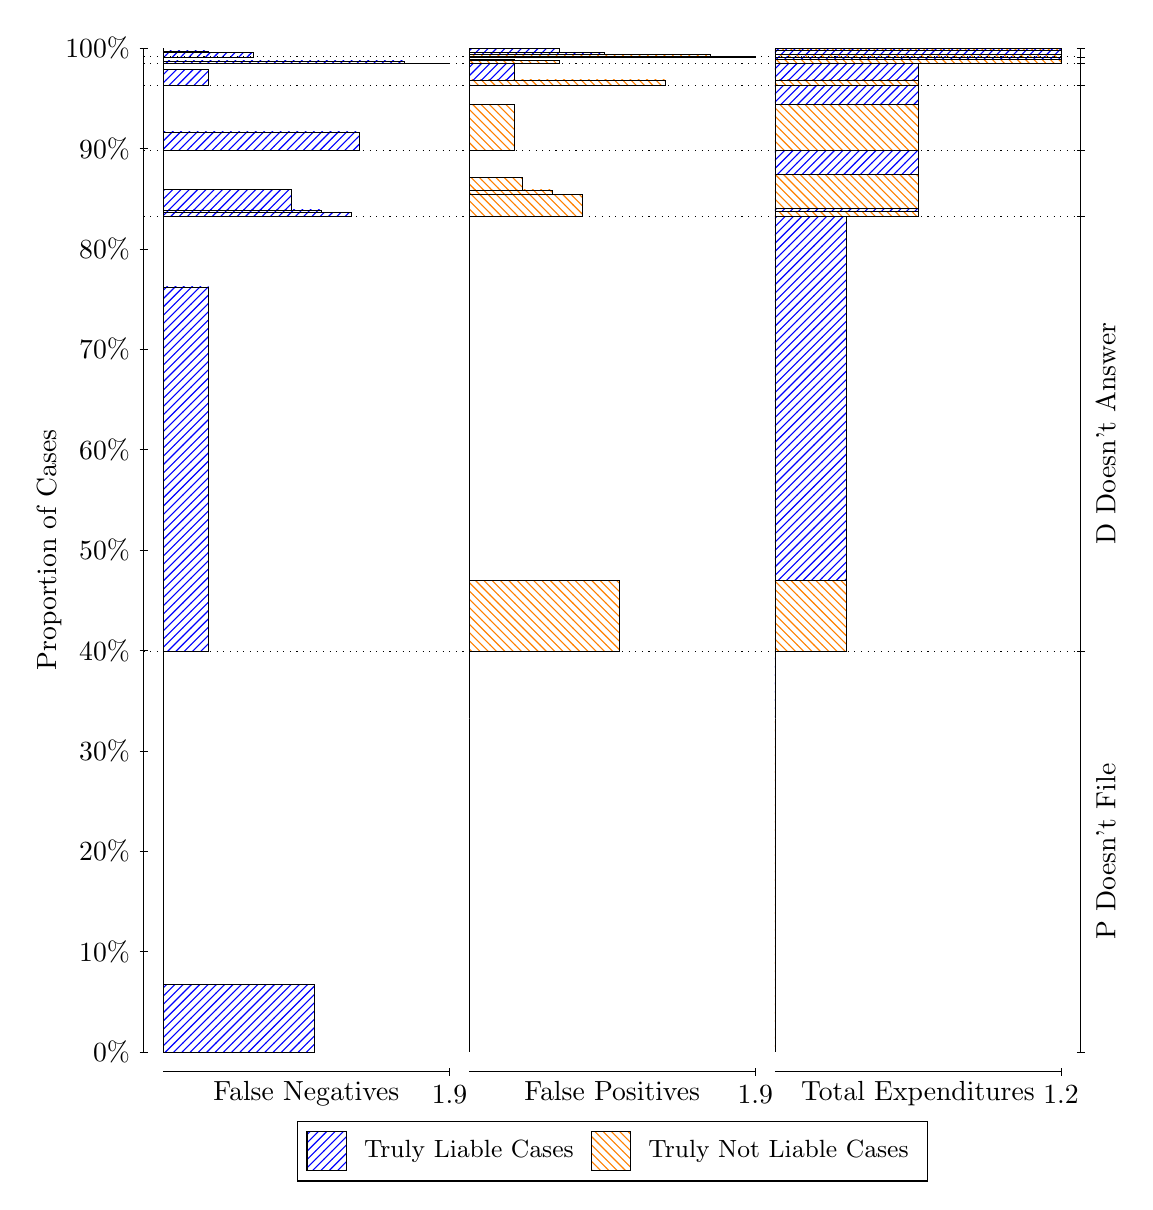
\begin{tikzpicture}
\draw[black, very thin] (1.5,1.75) -- (1.5,14.5);
\node[rotate=90, anchor=center] at (0.3, 8.125) {Proportion of Cases};
\draw[black, very thin] (1.45,1.75) -- (1.55,1.75);
\node[anchor=east] at (1.45, 1.75) {0\%};
\draw[black, very thin] (1.45,3.025) -- (1.55,3.025);
\node[anchor=east] at (1.45, 3.025) {10\%};
\draw[black, very thin] (1.45,4.3) -- (1.55,4.3);
\node[anchor=east] at (1.45, 4.3) {20\%};
\draw[black, very thin] (1.45,5.575) -- (1.55,5.575);
\node[anchor=east] at (1.45, 5.575) {30\%};
\draw[black, very thin] (1.45,6.85) -- (1.55,6.85);
\node[anchor=east] at (1.45, 6.85) {40\%};
\draw[black, very thin] (1.45,8.125) -- (1.55,8.125);
\node[anchor=east] at (1.45, 8.125) {50\%};
\draw[black, very thin] (1.45,9.4) -- (1.55,9.4);
\node[anchor=east] at (1.45, 9.4) {60\%};
\draw[black, very thin] (1.45,10.675) -- (1.55,10.675);
\node[anchor=east] at (1.45, 10.675) {70\%};
\draw[black, very thin] (1.45,11.95) -- (1.55,11.95);
\node[anchor=east] at (1.45, 11.95) {80\%};
\draw[black, very thin] (1.45,13.225) -- (1.55,13.225);
\node[anchor=east] at (1.45, 13.225) {90\%};
\draw[black, very thin] (1.45,14.5) -- (1.55,14.5);
\node[anchor=east] at (1.45, 14.5) {100\%};

\draw[black, very thin] (13.4,1.75) -- (13.4,14.5);
\draw[black, very thin] (13.35,1.75) -- (13.45,1.75);
\node[anchor=west] at (13.35, 1.75) {};
\draw[black, very thin] (13.35,6.8406) -- (13.45,6.8406);
\node[anchor=west] at (13.35, 6.8406) {};
\draw[black, very thin] (13.35,12.365) -- (13.45,12.365);
\node[anchor=west] at (13.35, 12.365) {};
\draw[black, very thin] (13.35,13.196) -- (13.45,13.196);
\node[anchor=west] at (13.35, 13.196) {};
\draw[black, very thin] (13.35,14.021) -- (13.45,14.021);
\node[anchor=west] at (13.35, 14.021) {};
\draw[black, very thin] (13.35,14.302) -- (13.45,14.302);
\node[anchor=west] at (13.35, 14.302) {};
\draw[black, very thin] (13.35,14.387) -- (13.45,14.387);
\node[anchor=west] at (13.35, 14.387) {};
\draw[black, very thin] (13.35,14.5) -- (13.45,14.5);
\node[anchor=west] at (13.35, 14.5) {};

\draw[black, very thin, pattern color=blue, pattern=north east lines] (1.75,1.75) rectangle (3.6623,2.6054);
\draw[black, very thin, pattern color=orange, pattern=north west lines] (1.75,2.6054) rectangle (1.75,6.8406);
\draw[black, very thin, pattern color=blue, pattern=north east lines] (1.75,6.8406) rectangle (2.3237,11.467);
\draw[black, very thin, pattern color=orange, pattern=north west lines] (1.75,11.467) rectangle (1.75,12.365);
\draw[black, very thin, pattern color=blue, pattern=north east lines] (1.75,12.365) rectangle (4.1404,12.408);
\draw[black, very thin, pattern color=blue, pattern=north east lines] (1.75,12.408) rectangle (3.7579,12.445);
\draw[black, very thin, pattern color=blue, pattern=north east lines] (1.75,12.445) rectangle (3.3754,12.702);
\draw[black, very thin, pattern color=orange, pattern=north west lines] (1.75,12.702) rectangle (1.75,13.196);
\draw[black, very thin, pattern color=blue, pattern=north east lines] (1.75,13.196) rectangle (4.236,13.434);
\draw[black, very thin, pattern color=orange, pattern=north west lines] (1.75,13.434) rectangle (1.75,14.021);
\draw[black, very thin, pattern color=blue, pattern=north east lines] (1.75,14.021) rectangle (2.3237,14.226);
\draw[black, very thin, pattern color=orange, pattern=north west lines] (1.75,14.226) rectangle (1.75,14.302);
\draw[black, very thin, pattern color=blue, pattern=north east lines] (1.75,14.302) rectangle (5.3833,14.306);
\draw[black, very thin, pattern color=blue, pattern=north east lines] (1.75,14.306) rectangle (4.8096,14.336);
\draw[black, very thin, pattern color=orange, pattern=north west lines] (1.75,14.336) rectangle (1.75,14.387);
\draw[black, very thin, pattern color=blue, pattern=north east lines] (1.75,14.387) rectangle (2.8974,14.442);
\draw[black, very thin, pattern color=blue, pattern=north east lines] (1.75,14.442) rectangle (2.3237,14.465);
\draw[black, very thin, pattern color=orange, pattern=north west lines] (1.75,14.465) rectangle (1.75,14.5);
\draw[black, very thin, pattern color=orange, pattern=north west lines] (5.6333,1.75) rectangle (5.6333,5.9852);
\draw[black, very thin, pattern color=blue, pattern=north east lines] (5.6333,5.9852) rectangle (5.6333,6.8406);
\draw[black, very thin, pattern color=orange, pattern=north west lines] (5.6333,6.8406) rectangle (7.5456,7.7388);
\draw[black, very thin, pattern color=blue, pattern=north east lines] (5.6333,7.7388) rectangle (5.6333,12.365);
\draw[black, very thin, pattern color=orange, pattern=north west lines] (5.6333,12.365) rectangle (7.0675,12.639);
\draw[black, very thin, pattern color=orange, pattern=north west lines] (5.6333,12.639) rectangle (6.6851,12.699);
\draw[black, very thin, pattern color=orange, pattern=north west lines] (5.6333,12.699) rectangle (6.3026,12.859);
\draw[black, very thin, pattern color=blue, pattern=north east lines] (5.6333,12.859) rectangle (5.6333,13.196);
\draw[black, very thin, pattern color=orange, pattern=north west lines] (5.6333,13.196) rectangle (6.207,13.782);
\draw[black, very thin, pattern color=blue, pattern=north east lines] (5.6333,13.782) rectangle (5.6333,14.021);
\draw[black, very thin, pattern color=orange, pattern=north west lines] (5.6333,14.021) rectangle (8.1193,14.096);
\draw[black, very thin, pattern color=blue, pattern=north east lines] (5.6333,14.096) rectangle (6.207,14.302);
\draw[black, very thin, pattern color=orange, pattern=north west lines] (5.6333,14.302) rectangle (6.7807,14.34);
\draw[black, very thin, pattern color=orange, pattern=north west lines] (5.6333,14.34) rectangle (6.207,14.353);
\draw[black, very thin, pattern color=blue, pattern=north east lines] (5.6333,14.353) rectangle (5.6333,14.387);
\draw[black, very thin, pattern color=orange, pattern=north west lines] (5.6333,14.387) rectangle (9.2667,14.393);
\draw[black, very thin, pattern color=orange, pattern=north west lines] (5.6333,14.393) rectangle (8.693,14.422);
\draw[black, very thin, pattern color=blue, pattern=north east lines] (5.6333,14.422) rectangle (7.3544,14.446);
\draw[black, very thin, pattern color=blue, pattern=north east lines] (5.6333,14.446) rectangle (6.7807,14.5);
\draw[black, very thin, pattern color=orange, pattern=north west lines] (9.5167,1.75) rectangle (9.5167,5.9852);
\draw[black, very thin, pattern color=blue, pattern=north east lines] (9.5167,5.9852) rectangle (9.5167,6.8406);
\draw[black, very thin, pattern color=orange, pattern=north west lines] (9.5167,6.8406) rectangle (10.425,7.7388);
\draw[black, very thin, pattern color=blue, pattern=north east lines] (9.5167,7.7388) rectangle (10.425,12.365);
\draw[black, very thin, pattern color=orange, pattern=north west lines] (9.5167,12.365) rectangle (11.333,12.425);
\draw[black, very thin, pattern color=blue, pattern=north east lines] (9.5167,12.425) rectangle (11.333,12.461);
\draw[black, very thin, pattern color=orange, pattern=north west lines] (9.5167,12.461) rectangle (11.333,12.895);
\draw[black, very thin, pattern color=blue, pattern=north east lines] (9.5167,12.895) rectangle (11.333,13.196);
\draw[black, very thin, pattern color=orange, pattern=north west lines] (9.5167,13.196) rectangle (11.333,13.782);
\draw[black, very thin, pattern color=blue, pattern=north east lines] (9.5167,13.782) rectangle (11.333,14.021);
\draw[black, very thin, pattern color=orange, pattern=north west lines] (9.5167,14.021) rectangle (11.333,14.096);
\draw[black, very thin, pattern color=blue, pattern=north east lines] (9.5167,14.096) rectangle (11.333,14.302);
\draw[black, very thin, pattern color=orange, pattern=north west lines] (9.5167,14.302) rectangle (13.15,14.353);
\draw[black, very thin, pattern color=blue, pattern=north east lines] (9.5167,14.353) rectangle (13.15,14.387);
\draw[black, very thin, pattern color=orange, pattern=north west lines] (9.5167,14.387) rectangle (13.15,14.417);
\draw[black, very thin, pattern color=blue, pattern=north east lines] (9.5167,14.417) rectangle (13.15,14.471);
\draw[black, very thin, pattern color=orange, pattern=north west lines] (9.5167,14.471) rectangle (13.15,14.476);
\draw[black, very thin, pattern color=blue, pattern=north east lines] (9.5167,14.476) rectangle (13.15,14.5);
\draw[black, dotted] (1.5,6.8406) -- (13.4,6.8406);
\draw[black, dotted] (1.5,12.365) -- (13.4,12.365);
\draw[black, dotted] (1.5,13.196) -- (13.4,13.196);
\draw[black, dotted] (1.5,14.021) -- (13.4,14.021);
\draw[black, dotted] (1.5,14.302) -- (13.4,14.302);
\draw[black, dotted] (1.5,14.387) -- (13.4,14.387);
\draw[black, very thin] (1.75,1.5) -- (5.3833,1.5);
\node[anchor=north] at (3.5667, 1.5) {False Negatives};
\draw[black, very thin] (5.3833,1.45) -- (5.3833,1.55);
\node[anchor=north] at (5.3833, 1.45) {1.9};

\draw[black, very thin] (5.6333,1.5) -- (9.2667,1.5);
\node[anchor=north] at (7.45, 1.5) {False Positives};
\draw[black, very thin] (9.2667,1.45) -- (9.2667,1.55);
\node[anchor=north] at (9.2667, 1.45) {1.9};

\draw[black, very thin] (9.5167,1.5) -- (13.15,1.5);
\node[anchor=north] at (11.333, 1.5) {Total Expenditures};
\draw[black, very thin] (13.15,1.45) -- (13.15,1.55);
\node[anchor=north] at (13.15, 1.45) {1.2};

\node[black, centered, rotate=90] at (13.72, 4.2953) {P Doesn't File};
\node[black, centered, rotate=90] at (13.72, 9.6027) {D Doesn't Answer};






\draw (7.449999999999999,1.5) node[draw=none] (baseCoordinate) {};
\begin{scope}[align=center]
        \matrix[scale=0.5, draw=black, below=0.5cm of baseCoordinate, nodes={draw}, column sep=0.1cm]{
            \node[rectangle, draw, minimum width=0.5cm, minimum height=0.5cm, pattern=north east lines, pattern color=blue] {}; &
            \node[draw=none, font=\small] (B) {Truly Liable Cases}; &
            \node[rectangle, draw, minimum width=0.5cm, minimum height=0.5cm, pattern=north west lines, pattern color=orange] {}; &
            \node[draw=none, font=\small] (B) {Truly Not Liable Cases}; \\
            };
\end{scope}

\end{tikzpicture}
\end{document}